\chapter{System Description}\label{chap:sys_description}
The present chapter covers the system design including specific solutions that have been chosen for the realization of the SmartNotes application. The system concept, introduced in chapter~\ref{chap:concept}, will become extended by describing certain elements of implementation and problems found during the development process. This should allow the reader have a deeper view into the SmartNotes application including functions that it offers and platform that it runs on.
\section{Google App Engine platform}\label{sec:gae}
Google App Engine seems to be an outstanding development platform. For all the reasons mentioned in~\ref{sec:gae_general}, it has been decided to be used as the main platform for SmartNotes before any other hosting services. Besides, GAE appears to be highly competitive in terms of cost calculations, which are described in section~\ref{subsec:gae_calculations}. After registering the application with a unique name, it can be easily uploaded to Google and after a few seconds it is accessible to its users.

*****As stressed in section~\ref{subsec:sync_scenarios} the synchronization scenarios use the client-server architecture. When running on GAE platform which is as mentioned in~\ref{sec:gae_general} distributed vault-tolerant infrastructure where two subsequent request may be served by different machines located in separate data-centers. Thus from the addressing scope the application can still be treated as centralized server. In case the application requires state awareness it is the developer role to make it so. Otherwise the fact that the application is served from multiple machines is completely transparent from the functional point of view of application. 

SmartNotes uses only some of the supported by GAE components. This ones which make a part of SmartNotes application with relation with some other third-party elements are presented on figure~\ref{fig:smartnotes_components}. This is especially important as it presents all the application top level components together with marked interfaces between the particular functional blocks. This diagram strongly corresponds with the diagram form figure~\ref{fig:ismartnotes_smartnotes} which in general way presents the cooperation of SmartNotes and iSmartNotes with differentiated roles of administrator and user. 

The most complicated structure is the SmartNotes component which is marked as an individual system. It does not require the iSmartNotes to realize its functionality. For this reason SmartNotes component could work with any kind of client application using the interface that it provides. This is the interface of Mercurial HTTP chains of requests and responses that needed a some back-end redesign to accommodate to the conditions set the GAE. The issues  connected with cooperation of Mercurial and Google app engine are the topic of section~\ref{sec:hg_on_gae}. Furthermore the SmartNotes uses thee additional interfaces which are used to interconnect the Google App Engine component with the Mercurial adopted to run on GAE and separately the admin and the user interfaces provided by SmartNotes. Each of this three components is connected in a different way. Whereas  webapp framework has  low Python overhead as mentioned in section~\ref{subsec:webapp} and was chosen to serve the connection between the Mercurial GAE component and the Google App Engine componet for performance reasons it is Django which is the best choice when it comes to building nontrivial web based functionality for reasons mentioned in section~\ref{subsec:django}. The remaining two elements used by Google App Engine subsystem are the Google Account and the Datastore. The role of the first one was with detail presented while discussing the iSmartNotes activation process in section~\ref{subsec:ismartnotes_activation}. Some of the Datastore details will be covered in section~\ref{sec:hg_on_gae}. 
\begin{figure}[ht]
\begin{center}
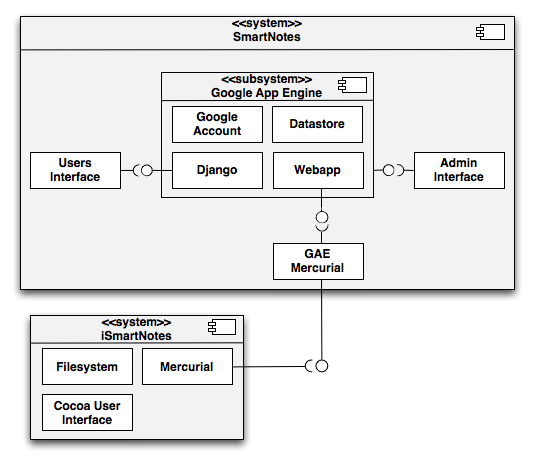
\includegraphics[scale=0.6]{charts/smartnotes_componets.png}
\caption{The components diagram of  the SmartNotes application with marked interfaces between the functional blocks.}
\label{fig:smartnotes_components}
\end{center}
\end{figure}

The second independent system is the iSmartNotes component. This one stay independent until the user decides to activate it to use synchronization feature. For this purpose it requires a Mercurial server to interact with.The iSmartNotes as presented on figure~\ref{fig:smartnotes_components} is build of three components. First one is the filesystem of the client operating system which is the classical space where Version Control Systems allocate their repositories. Secondly Mercurial VCS which on the client site does not require any modifications and finally the Cocoa user interface which presentation is dedicated section~\ref{sec:cocoa}.

\subsection{Financial calculations}\label{subsec:gae_calculations}
\section{Mercurial on Google App Engine}\label{sec:hg_on_gae}
\section{Cocoa user interface}\label{sec:cocoa}